\section{Deep Learning} \label{sec:bt/DNN}

Deep learning is a powerful extension of the simple learning algorithms detailed above. In theory, any problem which can be modeled as the mapping of an input vector to an output vector can be solved by deep learning \cite{goodfellow2016}. In other words, any function of any complexity can be approximated given sufficiently large models and sufficiently large labeled training examples. 

\subsection{Deep Feedforward Neural Networks}

Feedforward neural networks constitute a branch of deep learning covering models with a one-directional data flow from input to output. They are called \textit{neural networks} because they are loosely inspired by the neural circuitry of the human brain. Extending this analogy, all human perception may be considered one vast deep feedforward neural network. It works by mapping sensory input from sight, touch, smell, taste, and hearing through countless layers of neurons to output what we perceive of the world. Artificial neural networks work similarly by mapping a vector of input data points to one or more output values.

Even in their simplest form, deep feedforward neural networks overcome many challenges that linear models face. Linear regression, for instance, may never accurately approximate a non-linear function or capture interactions between two or more input variables. This limitation may only be overcome by introducing a nonlinearity to the input $\bm{x}$. We encapsulate this nonlinearity as $\phi(\bm{x})$. Thus, the equivalent to equation \ref{eq:bt_linReg} becomes equation \ref{eq:bt/dnn/dfnn}.

\begin{equation}
    \label{eq:bt/dnn/dfnn}
    y=f(\bm{x};\bm{\theta},\bm{x})=\phi(\bm{x};\bm{\theta})^T\bm{w}
\end{equation}

We now have another set of trainable parameters $\bm{\theta}$, meaning that the final form of $\phi$ is yet to be determined. By allowing the model to experience a given set of labeled training data, $\bm{\theta}$ will gradually converge towards a value that enables the full model to approximate the data optimally.
% be trained from experiencing a given set of labeled training data. 
The parameters defined by $\bm{w}$ may subsequently map from $\phi(\bm{x})$ to the desired output. $\phi$ is called a \textit{hidden layer} because its outputs are unrelated to either the input or output vectors. It can instead be thought of as a transformation of the input layer. 
% We can think of $\phi$ as a transformation of the input layer. 
Its output is hence a new representation or interpretation of the information provided by $\bm{x}$.

\begin{figure}[h]
    \centering
    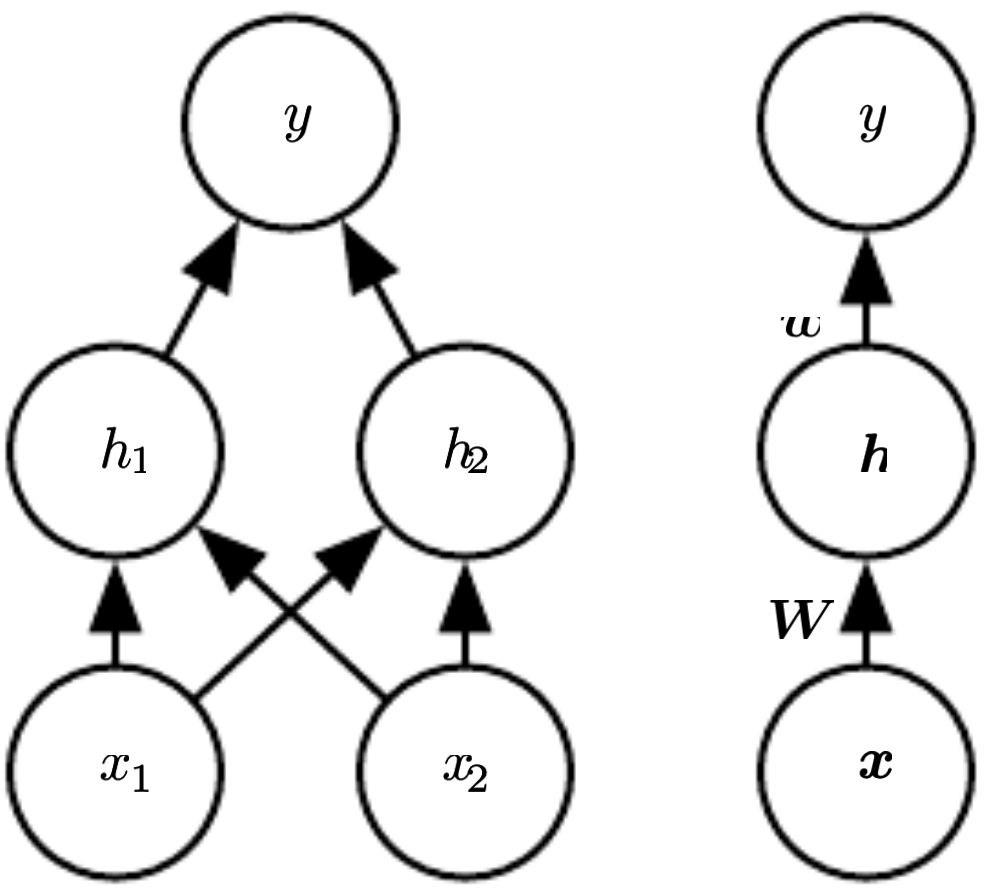
\includegraphics[width=0.5\textwidth]{figures/bt_dfnn.png}
    \caption{Example of a simple \acrshort{mlp}. Left representation depicts individual neurons of each layer and the edges between them. The right representation is more common, depicting each layer with vector notation. }
    \source{\cite{goodfellow2016}}
    \label{fig:bt_dfnn}
\end{figure}

\subsubsection{\acrlong{mlp}}

A \acrfull{mlp} is one form of feedforward neural network, the simplest implementation of which is illustrated in figure \ref{fig:bt_dfnn}. Here we have two input neurons, one hidden layer with two neurons, and one output layer with one neuron. With vector notation, we say that the hidden layer $\bm{h}$ is a function of the input layer $\bm{x}$, with the relation $\bm{h}=f^{(1)}(\bm{x};\bm{W}, \bm{c})$. $\bm{h}$ is then the input to a third layer (which in this case is also the output layer) with the relation $y=f^{(2)}(\bm{h};\bm{W}, \bm{c})$. We can keep adding depth and width to the model this way, further increasing its complexity and potential hypothesis space. The entire model may now be given by equation \ref{eq:bt/dnn/mlp1}.

\begin{equation}
    \label{eq:bt/dnn/mlp1}
    f(\bm{x};\bm{W},\bm{c},\bm{w},b)=f^{(2)}(f^{(1)}(\bm{x}))
\end{equation}

To provide the nonlinearity we want, we define $\bm{h}=g(\bm{W}^T\bm{x}+\bm{c})$. This functon is commonly known as the \textit{activation function} of the layer. For deeper networks, it would be added to the output of every hidden layer. There are many activation functions to choose from, but the default recommendation in the machine learning community is to use the \acrfull{relu} \cite{agarap2018}. It is defined as $g(z)=max\{0,z\}$ and has been made popular for its simplicity without trading off on optimization with gradient-based backpropagation. The complete network of figure \ref{fig:bt_dfnn} can thus be given by equation \ref{eq:bt/dnn/mlp3}.

\begin{equation}
    \label{eq:bt/dnn/mlp2}
    y=f(\bm{x};\bm{W},\bm{c}, \bm{w}, b)=\bm{w}^Tg(\bm{W}^T\bm{x}+\bm{c}) + b
\end{equation}

\begin{equation}
    \label{eq:bt/dnn/mlp3}
    y=f(\bm{x};\bm{W},\bm{c}, \bm{w}, b)=\bm{w}^Tmax\{\bm{W}^T\bm{x}+\bm{c}\} + b
\end{equation}

\newpage
\subsection{\acrlong{cnn}s} \label{sec:bt/DNN/CNN}

A \acrfull{cnn} is a specialized kind of deep feedforward neural network that has shown remarkable results in computer vision and language processing. When first proposed by \textcite{lecun1989} in 1989, it revolutionized machine learning problems where data had a grid-structured topology. Such data could be interpreted with more insight while allowing for much deeper and scaleable model architectures. Before its inception, most practitioners had little faith in the advent of neural networks for machine learning. The success of \acrshort{cnn}s triggered a wave of interest, which laid the foundation for further research in neural networks and deep learning \cite{goodfellow2016}.

\subsubsection{Convolution}

To understand \acrshort{cnn}s, we need to understand what a \textit{convolution} is. Used in many engineering disciplines, it is simply a mathematical operator which expresses how two functions overlap \cite{weisstein2003}. In signal processing, for instance, convolution may be used to mathematically replicate how a given sound signal would behave in any conceivable environment. All one would need is the impulse response of this environment, which could be the recording of a clap or similar fast transient sound. Convolving these two signals would have the effect of "placing" the sound in this environment, artificially reproducing all reverberations. The operation is typically denoted with an asterisk and is defined as equations \ref{eq:bt/dnn/conv1}-\ref{eq:bt/dnn/conv2}. This particular version is known as discrete convolution, which is what we will be encountering for neural networks.

\begin{equation}
    \label{eq:bt/dnn/conv1}
    s(t)=(x*k)(t)
\end{equation}

\begin{equation}
    \label{eq:bt/dnn/conv2}
    s(t)=\sum_{a=-\infty}^{\infty}x(a)k(t-a)
\end{equation}

With \acrshort{cnn} terminology, $x$ is the input to a convolutional layer and $k$ is its \textit{kernel}. Since the input to a \acrshort{cnn} is often an image, time series, or other signals, $x$ and $k$ are usually multidimensional. Taking image classification as an example, the convolutional operations performed on all input pixels would look like equation \ref{eq:bt/dnn/conv3}.

\begin{equation}
    \label{eq:bt/dnn/conv3}
    S(i,j)=(K*X)(i,j)=\sum_{m}^{}\sum_{n}^{}X(i-m,j-n)K(m,n)
\end{equation}

Each pixel is denoted by $i$ and $j$ for its spatial coordinate in the input image. The output from convolving a kernel $K$ with an image $X$ is called a \textit{feature map} because it is essentially a mapping to a new "image" where features represented by the kernel are highlighted. A visual representation of how a 2-dimensional convolutional operation may be applied to an input is displayed in figure \ref{fig:bt_conv}.

\begin{figure}[h]
    \centering
    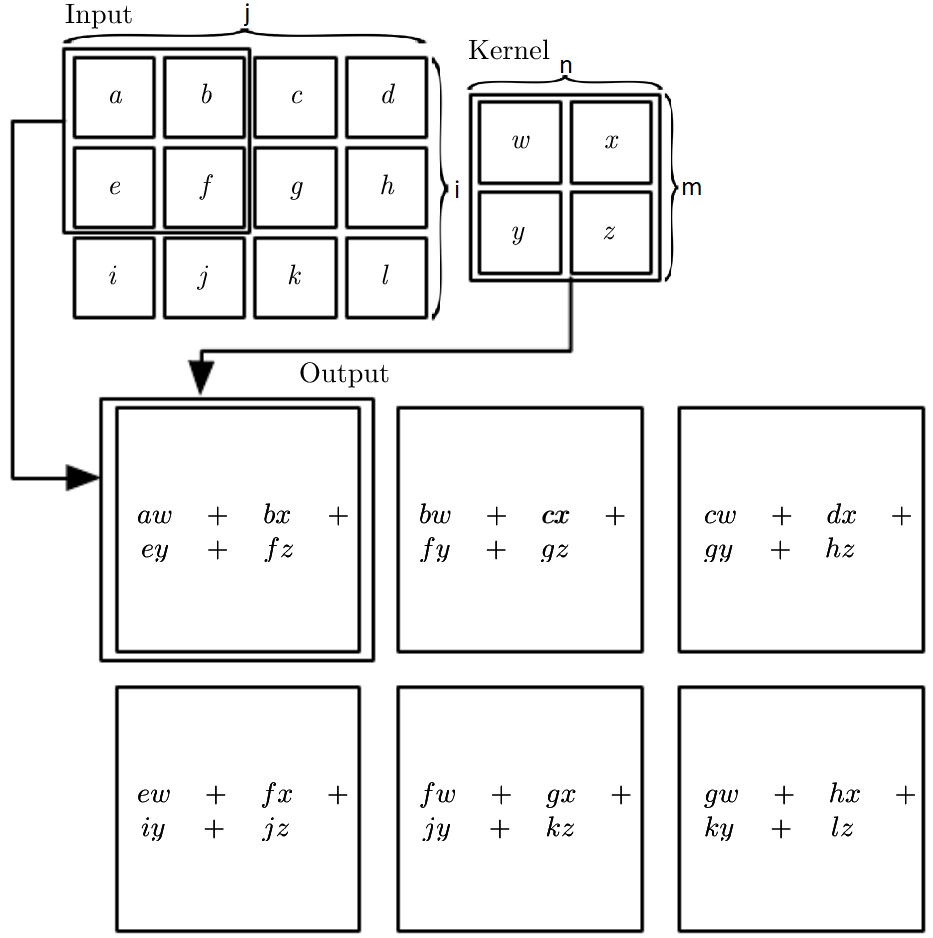
\includegraphics[width=0.8\textwidth]{figures/bt_conv.png}
    \caption{Example of 2-dimensional convolution operation. If this were image classification, values in the input matrix would represent individual pixel activations in the image. The final value of each output cell is calculated by the convolution operation given by equation \ref{eq:bt/dnn/conv3}.}
    \source{\cite{goodfellow2016}}
    \label{fig:bt_conv}
\end{figure}

The kernel $K$ is what defines all properties of a convolutional model. Instead of learning individual parameters for every edge between every neuron, as is the case for \acrshort{mlp}s, \acrshort{cnn}s learn the internal weights of all kernels in the network. As we will see, \acrshort{cnn}s usually contain several kernels for every convolutional layer, each capturing one feature in the input to each layer.

\subsubsection{Properties of \acrshort{cnn}s}

What makes \acrshort{cnn}s so efficient is based on three essential ideas. First, since parameters are only present in each kernel, as described above, the network does not need a single parameter for all neurons in every layer. This idea is known as \textit{parameter sharing} and will reduce the storage requirements of large models. Another consequence of the convolutional layers is that each input neuron is only connected to a few outputs. As can be seen in figure \ref{fig:bt_conv}, only four neurons of the input are required to calculate the value of a cell in the output. This idea is called \textit{sparse interactions}. Contrary to an \acrshort{mlp}, which requires connections from every input to every output, this feature drastically improves both computing efficiency and memory requirements during training.

Finally, a concept known as \textit{equivariant representations} allows for the detection of features that are independent of spatial (or temporal) position in the input. In other words, if there is an object in the input to a convolutional layer that causes high activations in a feature map, the same object will cause an equally high activation in the same feature map if it were in another position. This effect is another consequence of the way in which feature maps are created by "moving" the same kernel across the entire input. \acrshort{mlp}s, in contrast, lack this property since each neuron is associated with an individual learned weight. 
% The kernel will eventually reach and generate the convolutional output for that respective feature regardless of its po


% \subsection{Terms} \label{sec:bt/DNN/terms}

% Much machine learning terminology is considered common knowledge in most literature and is often neglected to be explained in detail. Some such terms, many of which will be used frequently during the course of this thesis, are detailed below.

% \subsubsection{Batch Normalization}
% \subsubsection{Dropout}
% % \subsubsection{Perceptron}
% % \subsubsection{\acrlong{relu}}
% \subsubsection{Max Pooling}
% \subsubsection{Softmax}
% \subsubsection{Cross Entropy Loss}
% \subsubsection{Precision, Accuracy and Recall}